% !TEX root = ../main.tex

\chapter{绪论}

\section{颗粒物质}

“当一个物体被分作几个单独运动的小部分时,它是液态的;而当它的所有部分都接触在一起时,它是固态的。” 这就是 17 世纪笛卡尔对于颗粒物质机械性质的朴素认知。颗粒物质在自然界中广泛存在,拥有可被类比于寻常物质所有的固(颗粒静堆积,也被称作 jammed state,即阻塞态)、液(颗粒流,也被称作 unjammed state,即非阻塞态)、气(颗粒分布均匀、快速运动)三态\cite{RevModPhys.68.1259},其共通特征是由离散物质构成的聚集系统,如沙漠、土壤、泥石流、沙尘暴;而在人类建设文明中,颗粒物质无疑也占有重要地位,如谷物堆积、矿石输运、药物粉末等生产行为,其背后也隐藏着颗粒堆积与流变的学问。即使是成本相对低廉的的煤炭、水泥、沙砾等工业材料,总共的生产与加工对地球上生产能源消耗的比例也来到了约 \num{10}\%\cite{duran2000sands}。因此对于颗粒物质的研究与理解,不仅有益于进一步认知自然界,从而防治地震、滑坡、雾霾、沙漠化等自然灾害,还有助于减少工业中的能源损失、预防粉尘爆炸等事故,进而提升人类工业文明的生产效率、提高生产质量。

颗粒物质的物理学是一门复杂的学科。颗粒物质通常被定义为尺度大于微米量级的宏观离散体,通过接触、碰撞等形式聚集组成的多体系统。颗粒物质拥有着丰富的物理特性,总结如下:

\begin{enumerate}
  \item 宏观性。足够的尺度与质量使得颗粒介质的运动无需考虑分子层面的热运动以及量子层面的概率分布效应,一种常见的分析思路是计算对比热力学尺度的 $k_{B}T$ 与颗粒尺度对应的引力势能 $mgd$,而常温($\sim$ 300 \unit{\kelvin})外部激励对于颗粒介质堆积结构的作用可以忽略(目前也的确存在对沙堆进行循环热剪切的相关实验\cite{YIN2023100503},但是这与我们论证不能通过温度遍历相空间的思路显然不同)。对于颗粒物理的力学研究也大多基于经典的牛顿力学;
  \item 离散性。在以等半径硬球组成的颗粒固体中,颗粒通常以随机的方式形成堆积,即介质中通常存在着空隙;对应地,使用体积分数 $\phi$ 来评估颗粒介质的空间利用率,其中对于等大硬球的情形存在着随机松散堆积(random loose packing,RLP)和随机密堆积(random close packing)两个体积分数极限,分别约为 0.55\cite{PhysRevLett.64.2727} 和 0.64\cite{RevModPhys.82.789}。随机性堆积的非晶结构使得传统的连续介质力学对颗粒介质的描述存在偏差\cite{RevModPhys.71.435};
  \item 多体性。三体问题已经是能产生混沌现象的复杂力学体系;即使只是静止状态下的颗粒固体,对于 $N$ 个颗粒进行描述也仍然需要多达 $3N$ 个正则坐标,即颗粒介质的多体特征使得其具有难以求解的极高自由度,所以对其进行宏观力学上的建模求解也是困难重重;
  \item 耗散性。颗粒间复杂的相互摩擦与碰撞使得系统中的各成员能迅速将动能转化为分子层面的热运动。因此颗粒系统中存在强耗散性,在失去外部能量驱动的情况下可以长期处于某一亚稳态(metastable state)。常规的统计力学假设,即系统在温度激励下可以遍历相空间中的微观态,对于颗粒介质而言失效。换言之,颗粒介质是典型的非平衡态系统;
  \item 敏感性。颗粒介质中存在高度复杂的力链与接触网络,而振动、剪切等外部激励容易使得颗粒进行重排(Rearrangement),使得这两种网络都具有高敏感性。因此对颗粒物质展开实验研究时,需要慎重考虑过程中的技术细节,避免观测手段本身对颗粒介质造成的扰动介入到所观察的实验现象中。
  \item 多分散性(polydispersity)。该术语原意是描述高分子聚合物的分子量不均一性,被援引至颗粒介质中用于指代多种不同颗粒的混合。虽然在大多数实验与理论中都是使用等大硬球模型来描述颗粒介质,但是在真实世界中的颗粒介质中,颗粒的尺寸、形状\cite{vandenwildenbergProbingEffectParticle2015,xingyi}、材料等参数不只是非均匀的,而且其在各自参数定义域上的分布也未必有规律,同时伴随着相分离\cite{doi:10.1126/sciadv.abe8737}等复杂动力学现象。
\end{enumerate}

颗粒物质的物理学也是年轻的学科。由于颗粒固体的弹性模量相较于通常的结晶固体要小得多,因此也被 de Gennes 将其与玻璃、液晶等体系共同称为“软物质”,并评论称“Granular matter, in 1998, is at the level of solid-state physics in 1930.”\cite{RevModPhys.71.S374}。2005 年 Science 提出的 125 个最重要前沿科学问题\cite{doi:10.1126/science.309.5731.78b}中,“能否发展关于湍流动力学和颗粒材料运动学的综合理论?”赫然在列;而 2021 年提出的 “新 125 个科学问题”\cite{sanders2021125}中,“集体运动的基本原理是什么?”仍然彰显着颗粒物质物理学的神秘。颗粒物理中的未知比已知多得多,虽然寻常但是蕴含着深刻的物理原理,亟待研究者们前赴后继的努力。

\section{颗粒物质的研究方法现状}


\subsection{实验方法}

针对颗粒物理中丰富的物理性质,目前已开发出多角度的实验研究方法。

\begin{enumerate}
  \item 光-弹性实验\cite{photoelasticimetry}。对于光学透明的介质,其内部应变时会展现出双折射现象,因此可以直观体现颗粒介质在受单轴剪切、环形剪切等外部作用下其内部的应力分布情形。但是由于偏振光在异质性介质中的传播、三维介质中的精确测量困难等问题\cite{Non-Destructive_3D_Photoelasticity},光弹性方法通常只适用于二维平面的颗粒介质;
  \item X 射线计算机断层扫描成像(computed tomography,CT)\cite{PhysRevE.68.020301}。X 射线扫描图像经由去边界、分水岭算法分割等处理后可以重构出颗粒介质的三维空间结构,从而研究颗粒介质中的接触结构与运动关系。但是该方法通常难以应用于实地实验。CT 设备本身成本已经较为昂贵,并且即使只是拍摄单张图像,其所需的存储空间也已较大(对于图像分辨率 $1021\times 1021 \times 886$,约占 $1.7\unit{\giga\byte}$ 的储存空间\cite{xujiazhao}),因此如果对实际测量时所拍摄的多帧图像进行数据处理,还需要配备价格不菲的高性能计算资源,进一步提高了其技术门槛。CT 设备由于射线源和探测板等性能限制,因此其空间分辨精度也会存在上限。这一点对于所研究颗粒的半径(为了得到图像中清晰的颗粒边界,一般要求颗粒的直径大于 $2\unit{\milli\meter}$)、材料(金属颗粒对 X 光吸收率过高而影响成像效果,因此不能被用于辐照)都存在一定限制。除此之外,一般的 X 光成像方法都是通过射线源和接收器对受辐照的物体进行旋转扫描以进行建模,这个拍摄过程通常会长达数十秒,所以对于高时间分辨需求的情境下,X 射线方法扫描建模方法不得不使用多源同步\cite{wang2008ultrafast}的方式间接提高时间分辨率;
  \item 核磁共振\cite{CLARKE2023}。另一类对颗粒介质进行成像研究的手段,只是“光源”换为了磁场。相应的,颗粒介质中需要对应的标记原子(这种原子核需要存在非零净磁矩,如最常用的质子成像就是利用的 H$^{1}$ 核),搭建对应的磁场线圈等也存在一定的技术门槛。
\end{enumerate}

以及本文所着眼的超声波探测技术。超声波在小振幅时具有非侵入式的探测作用,在有限振幅时则对颗粒介质具有诱导重排\cite{PhysRevE.84.020301}、流化/塑性软化(elastic weakening)\cite{PhysRevE.84.020301}等泵浦(pumping)作用。因此在设计超声波探测实验时,需要考虑其振幅、频率等参数与颗粒介质的相性。

超声波探测技术根据其探测思路可以大致分为两类:

\begin{enumerate}
  \item 主动探测。超声波在颗粒介质中的传播是对其内部应力与接触结构的直接体现\cite{PhysRevB.48.15646,Jia1999UltrasoundPI,Transitional}。超声波主动探测具有非侵入性、高灵敏度等优点;真实世界中的颗粒材料通常光学不透明或者剧烈光散射,使得超声波成为颗粒物质研究中独一无二的探针。对经由颗粒介质传播后的声信号进行频谱、波形、声速、衰减、相似性参数等分析,有助于研究颗粒介质内部的结构/应力特征;
  \item 被动探测。颗粒介质受剪切等外部激励时出现应力-应变曲线,这种宏观事件伴随着内部颗粒的重排、碰撞与摩擦等介观过程,这类机械过程会激发颗粒的机械振动,即发射出携带介观过程信息的声信号。这种振动事件被称为声发射(Acoustic Emission,AE)。通过分析 AE 信号的频谱、能量、波形、振动模密度等特征\cite{PhysRevLett.120.218003,10.1029/2023JB026612,doi:10.1073/pnas.2305134120},可以对颗粒介质受应力时的蠕变(creeping)、滞滑(stick-slip)事件等特征过程进行研究。
\end{enumerate}

声学探测的时间尺度相较于成像方法的小很多,在时间分辨率这一方面存在着天然的优势\cite{PhysRevE.84.020301},因此可以被设计用于剪切带探测\cite{PhysRevE.85.051302}等连续过程实验。


\subsection{理论方法}

虽然颗粒物质是典型的非平衡态系统,但是对其进行统计力学上的描述仍在争取中。在实验中已经发现,通过如图~\eqref{fig:apparatus_of_granular} 所示的振台振动、剪切盒循环剪切等外部激励方式操纵的颗粒堆积,其存在可重复的微观态;若进一步采取等概率假设,即相同体积颗粒堆积的微观结构概率相同,那么就可以将体积 $V$ 替代传统的统计力学中的哈密顿量 $H$,从而建立适用于颗粒物质的统计力学框架。Edwards 以这种思想提出了“等效温度”的定义\cite{EDWARDS19891080}:

\begin{figure}[!hbtp]
  \centering
  \bisubcaptionbox{控制加速度 $a$ 的振台装置}{Tapping experiment setup controlling the acceleration $a$}%
                [7cm]{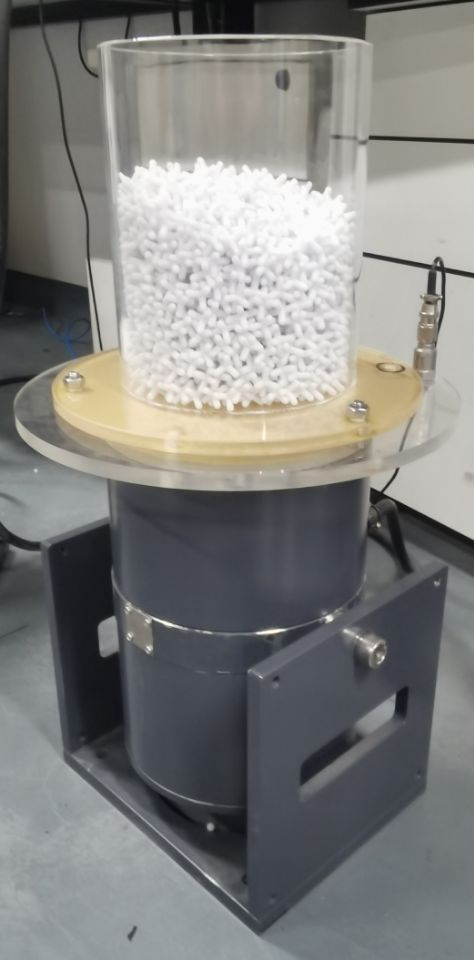
\includegraphics[height=6cm]{figures/1_tapping.jpg}}
  \hspace{1cm}
  \bisubcaptionbox{通过步进电机控制的剪切盒装置}{Shear box apparatus controlled by stepping motor}%
                [7cm]{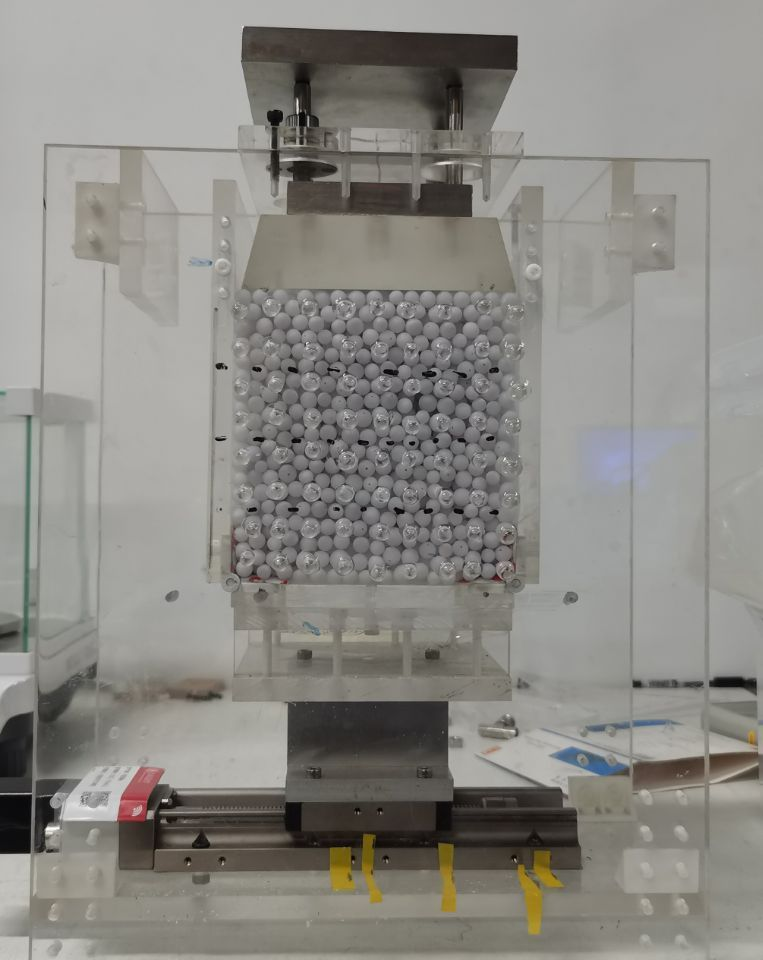
\includegraphics[height=6cm]{figures/1_shearing.jpg}}
  \bicaption{振台振动、剪切盒循环剪切等外部激励方式的装置示意图}{Schematic of the apparatus for external excitation methods such as tapping, cyclic shearing by the shear box, etc.}
  \label{fig:apparatus_of_granular}
\end{figure}

\begin{equation}
  \frac{1}{\chi} = \frac{\partial S(V)}{\partial V} = \frac{\partial \lambda\ln{\Omega(V)}}{\partial V},
\end{equation}

其中 $\chi$ 为等效温度(正式变量名为 Compactivity),$S$ 为熵,$\Omega(V)$ 是给定堆积体积 $V$ 下的微观态数目,$\lambda$ 是类比玻尔兹曼常数 $k_{B}$ 的常数。已有实验证明,这种定义的等效温度与通过涨落耗散效应定义的温度具有一致性\cite{PhysRevLett.129.228004}。

对于声学而言,在理论上依靠的主要是非线性声学\cite{10.1029/93JB02974}、等效介质理论(Effective Media Theory,EMT)\cite{WALTON1987213},依托于辐射传递方程(Radiative Transfer Equation,RTE)的扩散行为近似\cite{PhysRevLett.93.154303,PhysRevApplied.16.034009}。

\begin{figure}[!htp]
  \centering
  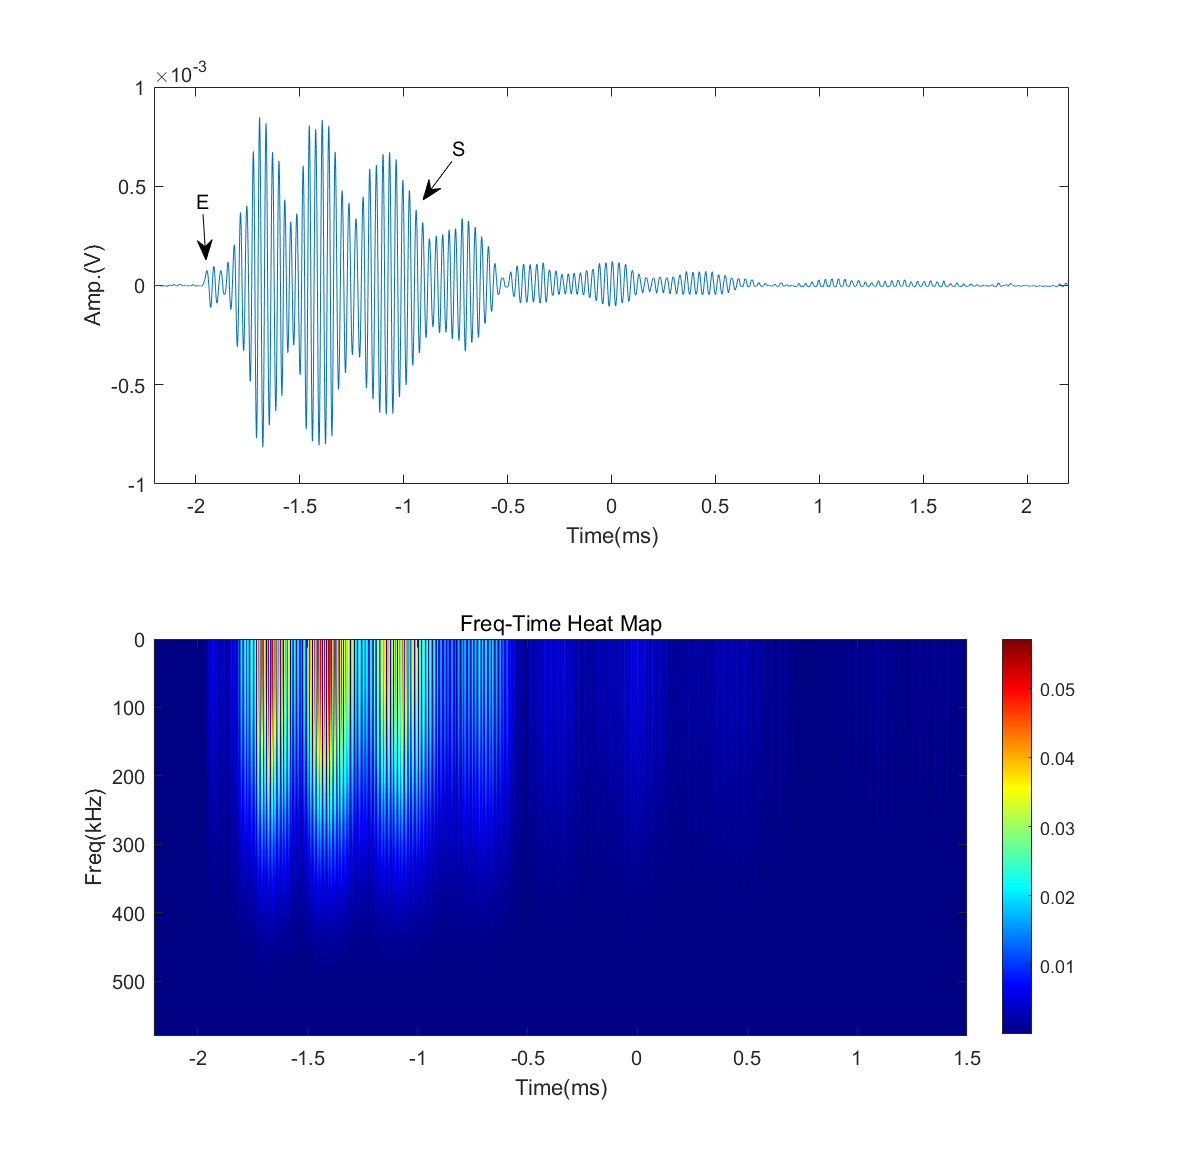
\includegraphics[height=10cm]{figures/1_heat_map.png}
  \bicaption{颗粒介质中典型的声信号。由相干首波(E)和散射尾波(S)组成。下图展示了声信号在时域上的各频率分量强度。}{Typical acoustic signal in granular media. It consists of a coherent first wave (E) and a scattering tail wave (S). The following figure illustrates the intensity of each frequency component in the acoustic signal along the time domain.}
  \label{fig:acoustic_signal}
\end{figure}

图~\ref{fig:acoustic_signal} 展示了超声波在颗粒固体中传播的示意图。可以观察到,超声波通常由相干弹性首波(Coherent Elastic Wave,简略为 E)与散射尾波(Codalike Scatter Wave,简略为 S)。 相干波是由颗粒介质中复杂力链自平均形成的,因此对应力与接触构型不敏感,而散射波则是对接触构型非常敏感,这一点与相干波完全相反\cite{PhysRevLett.93.154303}。

在连续介质力学中我们已经知道,三维介质中的波传播分为两种模式,即纵波/压缩波(Longitudinal Wave/Compressional Wave),以及横波/剪切波(Transverse Wave/Shear Wave)。这两种模式波引入到颗粒介质中时,即分别对应了其宏观统计性质的体弹性模量 $K$ 与剪切模量 $G$。EMT 理论综合了颗粒介质特有的体积分数 $\phi$、平均接触数/配位数 $Z$ 等物理量以及连续介质力学中的弹性模量,从而预测颗粒介质中不同模式的声速等物理量。

声学对于颗粒介质的研究范式大致可以根据等效波长 $\lambda_{\text{eff}} = V_{\text{eff}}/f_{c}$ 与振幅 $A$ 来进行总结分类。为方便我们记颗粒直径尺度为 $d$。

\begin{itemize}
  \item $\lambda_{E}\gg d$。此时关心的是在颗粒介质中的相干弹性波(coherent elastic waves)。由于此时颗粒介质的力学响应可以类比于寻常固体,所以 EMT 采用仿射变换近似(affine approximation)、平均场近似等方法将其处理为等效的连续介质。此时关心的是通常是横纵波速 $V_{P}$、$V_{S}$ 与等效介质弹性模量 $K$、$G$ 之间存在的关系。
  \item $\lambda_{E}\sim d$。此时声波在颗粒介质中的传播表现出强烈的多重散射特征。颗粒接触点的耗散性使得声波在颗粒介质中的衰减吸收大大加强了,因此研究者提出了扩散行为近似\cite{PhysRevLett.93.154303}、非线性波方程\cite{Transitional,hamilton_nonlinear_1998}等模型来对颗粒介质进行研究。在这些模型中,品质因子 $Q$、平均自由程 $l^{*}$ 等参数用于研究颗粒因接触点等因素产生的耗散性。
  \item $A\rightarrow 0$。对于小振幅声波,颗粒介质的非线性仅体现为其等效黏度 $\eta$ 等介质固有特征,且不会对颗粒介质的接触与应力结构造成显著影响。在此范围内我们将超声波视为非侵入性探针;
  \item $A\rightarrow \delta$。对于有限振幅声源,颗粒介质的非线性将被进一步激发,其等效黏度将会根据超声波振幅而产生变化,即声源激励已经对颗粒介质造成泵浦效果。比如利用超声波诱导倾斜面上的颗粒介质发生滑坡(landslide,avalanche)\cite{PhysRevE.102.042901},以及地震波诱导相邻地震成核(earthquake nucleation)区域的二次地震(co-seismic)\cite{Johnson_2005}等现象。
\end{itemize}

在本文中将使用激发与接收压缩波的成对声学探头,探究在不同应力和厚度下等大硬球颗粒介质对于超声波的响应情况,从而理解颗粒介质的内部结构与力学特性。

\section{本章小结}

本章介绍了颗粒物质的基本定义和丰富特性,以及目前在颗粒物理领域常见的实验和理论方法。在阐述了一般的声学研究范式后,我们将在以下的章节中详细展开相关实验,从而理解颗粒介质对于超声波的非线性响应。